\documentclass[11pt]{article}
\usepackage[margin=1in]{geometry}
\usepackage[T1]{fontenc}
\usepackage{lmodern}
\usepackage{booktabs,tabularx,graphicx,amsmath}
\usepackage[hidelinks]{hyperref}
\usepackage[font=small,labelfont=bf]{caption}
\usepackage{enumitem}
\usepackage{eurosym}
\setlist{nosep,leftmargin=1.2em}
\setlength{\parskip}{3pt}
\sloppy

\title{\vspace{-1.6em}\textbf{Small Model, Honest Numbers: A Distilled, Vocabulary-Pruned DeBERTa-v3-xsmall for RTE}}
\author{[Student name] \quad [Roll number] \quad CS6315E Neural Networks and Deep Learning\\
\small Code and predictions: submitted with this report (see the README)}
\date{\vspace{-2em}}

\begin{document}
\maketitle

\vspace{-1.2em}\section{Approach}
\textbf{Model choice.} Since accuracy is weighed against size, I compared three sizes of one pretrained family, DeBERTa-v3~\cite{he2021deberta,he2023debertav3} (base 184M, small 142M, xsmall 71M), with identical code. v3-base is my reference baseline and the distillation teacher; v3-xsmall is the student.

\textbf{Fine-tuning protocol.} One config-driven training path for all models: AdamW, 10\% linear warm-up then decay, layer-wise LR decay 0.9, separate head LR, max length 256, batch 16, early stopping on validation accuracy. With 2,490 training pairs results swing with the seed~\cite{mosbach2021stability}, so every configuration uses 5 seeds (mean $\pm$ sd). All decisions (early stopping, checkpoint and model selection, pruning level) use a 10\% validation split of train that is \emph{grouped by premise}, so near-duplicate pairs never straddle it. The dev set (277) is used only to report.

\textbf{Distillation.} Teacher soft labels are computed \emph{out-of-fold}: five DeBERTa-v3-base models, each trained on four premise-grouped folds, predict the fifth (OOF accuracy 82.9\%). The student minimises $\alpha\,\mathrm{CE}(y, s) + (1-\alpha)\,T^2\,\mathrm{KL}(\sigma(t/T)\,\|\,\sigma(s/T))$~\cite{hinton2015distilling} with $\alpha{=}0.5$, $T{=}2$, plus two variants: \emph{masked} KD (pure CE on rows where the teacher's argmax is wrong) and $\alpha{=}0.8$, $T{=}4$.

\textbf{Vocabulary pruning.} 49.2M of xsmall's 70.8M parameters are the $128{,}100\times384$ word embedding, yet RTE uses about 19k tokens. After training, I keep only the embedding rows of: special tokens $\cup$ every training-set token $\cup$ the top-$N$ tokens ranked by the tokenizer's own unigram log-probabilities~\cite{kudo2018subword}; all other ids map to \texttt{[UNK]} through a fixed lookup table~\cite{abdaoui2020load}. On input made only of kept tokens the pruned model is \emph{exactly} the original. $N$ is chosen on train alone: the smallest $N$ for which one half of train covers 98\% of the other half's tokens (giving $N{=}60{,}000$, 62,245 rows kept). I also tried a rank-128 SVD factorisation of the embedding (38.1M parameters).

\section{Results}
\begin{table}[h]
\centering\small
\begin{tabularx}{\linewidth}{@{}Xrrrr@{}}
\toprule
Model & Total params & Non-emb. & Dev acc.\ (5 seeds) & Val acc. \\
\midrule
Majority / word overlap / TF-IDF + LR & -- & -- & 52.7 / 57.4 / 57.0 & -- \\
DeBERTa-v3-base (my baseline, teacher) & 184.4M & 86.0M & $84.8 \pm 1.1$ & 86.2 \\
DeBERTa-v3-small & 141.9M & 43.5M & $76.5 \pm 1.4$ & 75.1 \\
DeBERTa-v3-xsmall, plain fine-tuning & 70.8M & 21.6M & $77.7 \pm 2.1$ & 78.5 \\
\quad + KD ($\alpha$ 0.5, $T$ 2) & 70.8M & 21.6M & $76.8 \pm 1.6$ & 78.4 \\
\quad + masked KD ($\alpha$ 0.5, $T$ 2) & 70.8M & 21.6M & $78.3 \pm 1.4$ & 79.2 \\
\quad + KD ($\alpha$ 0.8, $T$ 4) & 70.8M & 21.6M & $77.3 \pm 0.8$ & 79.5 \\
\quad rank-128 factorised embedding & 38.1M & 21.6M & $51.0 \pm 5.0$ & 57.6 \\
\midrule
\multicolumn{5}{@{}l}{\emph{Submitted (one checkpoint each, all DeBERTa-v3-xsmall):}} \\
\textbf{A}: masked KD, seed 21 & 70.8M & 21.6M & 78.0 & \textbf{82.7} \\
\textbf{B}: A, vocabulary-pruned & \textbf{45.5M} & 21.6M & 78.3 & 79.8$^\dagger$ \\
\textbf{C}: plain fine-tuning, seed 21 & 70.8M & 21.6M & 80.9 & 81.0 \\
\bottomrule
\end{tabularx}
\caption{GLUE RTE dev accuracy (\%). ``Val'' (premise-grouped validation split of train; mean of best epoch over seeds, or the checkpoint's own seed) is the only number used to choose anything. $^\dagger$Validation with only the tokens of the rows the model was fit on, so the text is unseen (Sec.~\ref{sec:select}).}
\label{tab:results}
\end{table}

Model B has \textbf{4.0$\times$ fewer parameters} than DeBERTa-v3-base (45.5M vs.\ 184.4M) and is 7.2 points lower on dev (85.6 vs.\ 78.3 for the selected checkpoints; McNemar $p{=}0.012$). A Colab rerun of seed 21 reproduced checkpoint A bit for bit; an Apple-MPS rerun did not (dev 74.7).

\textbf{Plain distillation copies the teacher's bias; masking it out helps a little.} KD at $\alpha{=}0.5$ scored $-0.9$ points versus plain fine-tuning (paired $t$ over seeds, $p{=}0.27$). It improved calibration (dev log-loss 0.74 vs.\ 0.99) and seed agreement (92\% vs.\ 88\%), but the teacher is biased: on train it predicts \emph{entailment} for 57.8\% of pairs against 50.2\% gold, and 72\% of its OOF errors are on not-entailment pairs. The KD student inherits it (61.5\% entailment predictions on dev vs.\ 52.7\% gold). Masked KD removes the inherited bias (55.8\%, same as plain) and is the best method on both dev ($+0.6$) and validation ($+0.7$), but neither gain is significant over 5 seeds ($p{=}0.57$, $0.21$). $\alpha{=}0.8$, $T{=}4$ has the best mean validation (79.5) and the lowest seed spread ($\pm0.8$) but not better dev.

\section{Accuracy vs.\ parameters: choosing three models}\label{sec:select}
\begin{figure}[h]
\centering
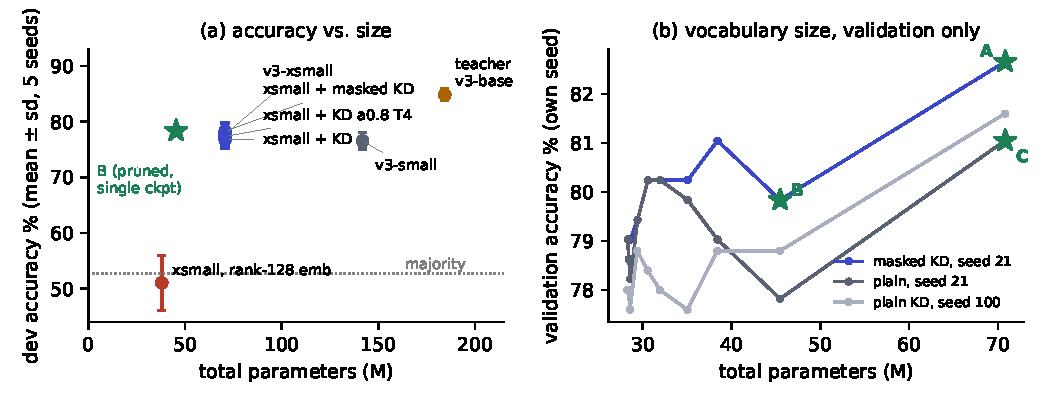
\includegraphics[width=0.94\linewidth]{figures/acc_vs_params.pdf}\vspace{-0.6em}
\caption{(a) Dev accuracy (mean $\pm$ sd over 5 seeds) against total parameters; the star is model B. (b) Validation accuracy of three checkpoints as the vocabulary shrinks (fit-split tokens + top-$N$ frequent, $N \in \{0,\dots,60\text{k},\text{all}\}$); stars are the submitted models.}
\label{fig:params}
\end{figure}

\textbf{Is a bigger model worth it?} Not within reach of xsmall (Fig.~\ref{fig:params}a): v3-small doubles every parameter count yet scored lower on validation (75.1 vs.\ 78.5) and dev. v3-base buys +7 points for 2.6$\times$ the parameters but is a different (wider, deeper) architecture, and the three submissions must share one; xsmall gives the best accuracy per parameter. Factorising its embedding (rank-128 SVD, 38.1M) destroyed it: training loss stayed at chance and dev fell to 51.0.

\textbf{Decision rule (validation only).} \textbf{A}: the highest-validation checkpoint of all 20 xsmall runs (masked KD, seed 21; 82.7). \textbf{B}: A with the pruned vocabulary, the one place where parameters clearly are not paying (36\% of them). Measuring that honestly needs care: the kept set contains every train token, validation rows included, so I re-score each checkpoint's validation split keeping only the tokens of the rows it was \emph{fit} on (Fig.~\ref{fig:params}b). The full vocabulary is best for all three checkpoints, by 2--3 points; with $n{\approx}248$ the standard error is $\pm2.5$ points, and on dev pruning moved accuracy by $+0.4$ and $-0.7$. So B trades $-36\%$ parameters for an estimated 0--3 points, and $N{=}60$k stays the train-only choice: picking the 38M peak would fit noise of one or two pairs. Keeping only training tokens (28.7M) costs 4 points on dev. \textbf{C}: the best checkpoint trained \emph{without} the teacher (plain, seed 21; 81.0), a hedge with different errors (it disagrees with A on 18 dev pairs; the best of A/B/C per pair would reach 84.1\%). If accuracy alone counts, A is my pick; per parameter, B.

\section{Error analysis}
Model B makes 60 errors on dev. 34 are false \emph{entailment} predictions (error rate 26.0\% on gold not-entailment vs.\ 17.8\% on entailment); it still predicts entailment slightly too often (55.6\% vs.\ 52.7\% gold). Automatic tags, error rate on each subset (overall 21.7\%): high lexical overlap ($\geq$80\%) but not entailed 36.8\% ($n{=}38$); low overlap ($<$50\%) but entailed 42.9\% (14); numbers/dates in the hypothesis 31.2\% (48); negation in exactly one side 22.5\% (40); top-10\% long premises 21.4\% (28). Negation and length are \emph{not} major error sources here.

I hand-labelled a random sample of 25 errors (seed 0; \texttt{report/error\_annotation.csv}):
\begin{itemize}
\item \textbf{Overlap, unsupported claim (7, all false entailments).} The hypothesis reuses premise words but changes a role or adds a detail: Mr Dean released a plan ``on behalf of the Secretary'' $\to$ ``Mr Dean is the Secretary''; ``a substance found in red wine'' $\to$ ``red wine''; an added ``60 million barrels''. This is the lexical-overlap heuristic known from NLI models~\cite{mccoy2019right}.
\item \textbf{Paraphrase missed (5, false non-entailments).} ``will spread out over a year'' $\to$ ``lasts a year''; ``BSE, the so-called mad cow disease''.
\item \textbf{Numbers (5).} Binding: 80\% approval belongs to Mrs.\ not Mr.\ Bush; 32 \emph{populations} read as 32 pandas. Comparison: \euro72.090.405,19 $>$ ``more than 72 million''; 12,000 years ago $\Rightarrow$ humans existed 10,000 years ago.
\item \textbf{Modality and world knowledge (6).} ``nearly 4 percent'' $\to$ ``4 percent''; ``attempt'' Everest $\to$ ``succeeds''; asked to form a government $\Rightarrow$ prime minister; once the model used outside knowledge the premise does not state (Bush's wife is Laura).
\item \textbf{Other (2):} one near the threshold ($p{=}0.39$), one doubtful gold label (a state court read as the U.S.\ Supreme Court).
\end{itemize}

\section{Reflection}
Counting \emph{where} the parameters are paid off most: vocabulary pruning is cheap and exact on covered text, though not free on unseen text. Distillation helped only once the teacher's wrong labels were masked, and then within seed noise; a factorised embedding and a bigger student did not help. \textbf{With more time/compute:} (i) prune the vocabulary \emph{before} fine-tuning and use the saved budget for a wider backbone; (ii) intermediate-layer or attention distillation instead of logits only, with the teacher's entailment bias corrected (class re-weighting or temperature per class); (iii) train-only data augmentation targeting the error classes above (role swaps, modality and quantifier edits of training hypotheses as not-entailment); (iv) more seeds to tighten the $\pm2$-point seed spread, larger than most effects here.

\textbf{Reproducibility.} Pinned \texttt{uv} env; each run stores config, versions, parameter counts, per-seed results; Colab reruns are bit-identical. \texttt{make train-submission submission} rebuilds A and B; \texttt{scripts/predict\_test.py} runs all three.

\small
\begin{thebibliography}{9}\setlength{\itemsep}{0pt}
\bibitem{abdaoui2020load} A.~Abdaoui, C.~Pradel, G.~Sigel. Load What You Need: Smaller Versions of Multilingual BERT. \emph{SustaiNLP}, 2020.
\bibitem{he2021deberta} P.~He, X.~Liu, J.~Gao, W.~Chen. DeBERTa: Decoding-enhanced BERT with Disentangled Attention. \emph{ICLR}, 2021.
\bibitem{he2023debertav3} P.~He, J.~Gao, W.~Chen. DeBERTaV3: Improving DeBERTa using ELECTRA-Style Pre-Training with Gradient-Disentangled Embedding Sharing. \emph{ICLR}, 2023.
\bibitem{hinton2015distilling} G.~Hinton, O.~Vinyals, J.~Dean. Distilling the Knowledge in a Neural Network. \emph{arXiv:1503.02531}, 2015.
\bibitem{kudo2018subword} T.~Kudo. Subword Regularization: Improving Neural Network Translation Models with Multiple Subword Candidates. \emph{ACL}, 2018.
\bibitem{mccoy2019right} R.~T.~McCoy, E.~Pavlick, T.~Linzen. Right for the Wrong Reasons: Diagnosing Syntactic Heuristics in Natural Language Inference. \emph{ACL}, 2019.
\bibitem{mosbach2021stability} M.~Mosbach, M.~Andriushchenko, D.~Klakow. On the Stability of Fine-tuning BERT. \emph{ICLR}, 2021.
\end{thebibliography}
\end{document}
